\section{Lecture 2: Lagrangian Mechanics, Euler-Lagrange Equations, and Hamiltonians}

\subsection{Lagrangian Mechanics and the Euler-Lagrange Equations}

We now consider a simplification of the previous lecture: we assume that the forces 
$\mathbf{F}_\alpha$ acting on the system are conservative.

\begin{definition}[Conservative Force]
A force $\mathbf{F}_\alpha$ is said to be \textbf{conservative} if the line integral of 
the force over any closed path is zero:

\begin{equation}
    \oint \mathbf{F}_\alpha \cdot d\mathbf{r}_\alpha = 0
\end{equation}

\end{definition}

This implies that the work done by the force in moving a particle between two points is 
independent of the path taken.  A conservative force can be expressed as the negative 
gradient of a scalar potential function $V$:

\begin{align}
    \mathbf{F}_\alpha &= -\mathbf{\nabla}_\alpha V(\mathbf{r}_1,\ \dots,\ \mathbf{r}_\alpha) \\
    &= - \frac{\partial}{\partial \mathbf{r}_\alpha} V(\mathbf{r}_1,\ \dots,\ \mathbf{r}_\alpha)
\end{align}

The work done in moving a particle from $\mathbf{r}_\alpha$ to $\mathbf{r}_\alpha'$ is 
given by $V(\mathbf{r}_\alpha) - V(\mathbf{r}_\alpha')$. In this course, we will 
primarily consider systems with conservative forces.

Since $\mathbf{r}_\alpha=\mathbf{r}_\alpha(q_i, t)$, the potential energy 
$V(\mathbf{r}_\alpha)$ can also be written as a function of the generalized coordinates:

\begin{equation}
    V(\mathbf{r}_\alpha)=V(q_i, t)
\end{equation}

Using the chain rule, we obtain:

\begin{equation}
    \frac{\partial V}{\partial q_i}=\sum_\alpha \frac{\partial V}{\partial \mathbf{r}_\alpha} \cdot \frac{\partial \mathbf{r}_\alpha}{\partial q_i}=-\sum_\alpha \mathbf{F}_\alpha \cdot \frac{\partial \mathbf{r}_\alpha}{\partial q_i}=-F_i
\end{equation}

Where $F_i$ is the generalized force corresponding to the generalized coordinate $q_i$.
From the previous lecture, we know that

\begin{equation}
   F_i = \frac{d}{dt} \left(\frac {\partial T}{\partial \dot{q_i}}\right) - \frac{\partial T}{\partial q_i}
\end{equation}

Therefore, for a conservative force, we can write:

\begin{equation}
    \frac{d}{dt} \left(\frac{\partial T}{\partial \dot{q}_i}\right) - \frac{\partial T}{\partial q_i} = -\frac{\partial V}{\partial q_i}
\end{equation}

Since the potential energy $V$ is not a function of $\dot{q}_i$, we have:

\begin{equation}
    \frac{\partial V}{\partial \dot{q}_i}=0
\end{equation}

We can now define the \textbf{Lagrangian} as $L = T - V$, where 
$L = L(q_i, \dot{q}_i, t)$. The equation of motion can then be rewritten as:

\begin{equation}
    \frac{d}{dt} \left(\frac{\partial L}{\partial \dot{q}_i}\right) - \frac{\partial L}{\partial q_i} = 0
\end{equation}

These are the \textbf{Euler-Lagrange Equations}. This set of equations provides a 
powerful means to obtain the equations of motion for a mechanical system using the 
Lagrangian.

These are $N$ differential equations, one for each degree of freedom. Typically, these 
are second-order ordinary differential equations (ODEs) for $q_i$.

In summary, given a system with $M$ particles and $N$ degrees of freedom, the following 
steps should be followed to determine the equations of motion using Lagrangian Mechanics:

\begin{enumerate}
    \item Identify the generalized coordinates $q_i$ that specify the system's 
    configuration, and express the position vectors of the particles as 
    $\mathbf{r}_\alpha=\mathbf{r}_\alpha(q_i, t)$, where $\alpha = 1, 2, \dots, M$ and 
    $i = 1, 2, \dots, N$.
    \item Calculate the kinetic energy 
    $T = \sum_\alpha \frac{1}{2} m_\alpha \dot{\mathbf{r}}_\alpha \cdot \dot{\mathbf{r}}_\alpha$ 
    as a function of $q_i$ and $\dot{q}_i$.
    \item Compute the potential energy $V = V(\mathbf{r}_\alpha) = V(q_i, t)$.
    \item Construct the Lagrangian $L = T - V$.
    \item Apply the Euler-Lagrange equations: 
    $\frac{d}{dt} \left(\frac{\partial L}{\partial \dot{q}_i}\right) - \frac{\partial L}{\partial q_i} = 0$.
\end{enumerate}

\begin{figure}[ht]
    \centering
    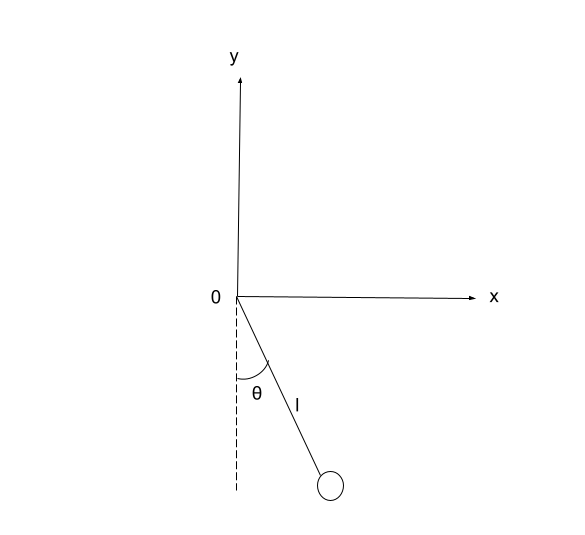
\includegraphics[width=0.4\textwidth]{images/2-1-1.png}
    \caption{Simple Pendulum Example}
    \label{fig:2-1-1}
\end{figure}

\begin{example}
    In Figure \ref{fig:2-1-1}, we have a simple pendulum with a mass $m$ and length $l$.
    Compute the equations of motion for the pendulum using Lagrangian mechanics.
    \label{ex:2-1}
\end{example}

As an example, let's consider the simple pendulum depicted in Figure \ref{fig:2-1-1}. 
The position of the pendulum bob can be written as:

\begin{align}
    x &= l \sin{\theta} \\
    y &= -l \cos{\theta} 
\end{align}

The time derivatives of the coordinates are:

\begin{align}
    \label{eq:2-12}
    \dot{x} &= l \cos{\theta} \cdot \dot{\theta} \\
    \label{eq:2-13}
    \dot{y} &= l \sin{\theta} \cdot \dot{\theta} 
\end{align}

Thus, the kinetic energy is:

\begin{equation}
    T=\frac{1}{2} m \left(\dot{x}^2+\dot{y}^2\right) = \frac{1}{2} ml^2\dot{\theta}^2
\end{equation}

The potential energy is:

\begin{equation}
    V=-mgy=-mgl\cos{\theta}
\end{equation}

The Lagrangian for the pendulum is:

\begin{equation}
    L=T-V=\frac{1}{2}ml^2\dot{\theta}^2+mgl\cos{\theta}
\end{equation}

Applying the Euler-Lagrange equation we get:

\begin{equation}
    \frac{d}{dt}\left(\frac{\partial L}{\partial\dot{\theta}}\right) - \frac{\partial L}{\partial\theta} = \frac{d}{dt}(ml^2\dot{\theta}) - (-mgl\sin{\theta})=ml^2\ddot{\theta}+mgl\sin{\theta}=0
\end{equation}

Thus the equation of motion of the simple pendulum is:

\begin{equation}
    ml^2\ddot{\theta}+mgl\sin{\theta}=0
\end{equation}

This result is consistent with what is obtained using Newton's laws of motion.

\subsection{Hamiltonian Mechanics}

While Lagrangian mechanics is conceptually valuable, we can take a further step by 
introducing the \textbf{Hamiltonian}. For a system with dynamical variables $q_i$ and a 
Lagrangian $L(q_i, \dot{q}_i, t)$, we define the Hamiltonian $H$ as:

\begin{equation}
    H=\sum_i \dot{q_i} \frac{\partial L}{\partial \dot{q_i}} - L
\end{equation}

Let's compute the total time derivative of the Hamiltonian:

\begin{align}
   \frac{dH}{dt}&=\sum_i \left(\ddot{q_i} \frac{\partial L}{\partial \dot{q_i}} + \dot{q_i} \frac{d}{dt} \left(\frac{\partial L}{\partial \dot{q_i}}\right)\right) - \sum_i \left(\frac{\partial L}{\partial q_i} \dot{q_i} + \frac{\partial L}{\partial \dot{q_i}} \ddot{q_i} \right) - \frac{\partial L}{\partial t}\\
   &=\sum_i\dot{q_i}\left(\frac{d}{dt} \left(\frac{\partial L}{\partial \dot{q_i}}\right)-\frac{\partial L}{\partial q_i}\right)-\frac{\partial L}{\partial t}
\end{align}

Using the Euler-Lagrange equation, we have:

\begin{equation}
    \frac{\partial L}{\partial q_i}=\frac{d}{dt} \left(\frac{\partial L}{\partial \dot{q_i}}\right)
\end{equation}

Thus, the equation simplifies to:

\begin{equation}
    \frac{dH}{dt}=-\frac{\partial L}{\partial t}
\end{equation}

The total time derivative of the Hamiltonian is the negative of the partial time 
derivative of the Lagrangian. If $L$ has no explicit time dependence, then:

\begin{equation}
    \frac{dH}{dt}=0
\end{equation}

This implies that $H$ is a conserved quantity.

What is the \textbf{Hamiltonian} physically? If the constraints are time-independent, then $\mathbf{r}_\alpha = \mathbf{r}_\alpha(q_i)$, and we have:

\begin{equation}
    T=\frac{1}{2} \sum_\alpha m_\alpha \dot{\mathbf{r}}_\alpha \cdot \dot{\mathbf{r}}_\alpha
\end{equation}

We can then compute

\begin{equation}
    \frac{\partial L}{\partial \dot{q_i}} = \frac{\partial T}{\partial \dot{q_i}} = \sum_\alpha m_\alpha \dot{\mathbf{r}}_\alpha \cdot \frac{\partial \dot{\mathbf{r}}_\alpha}{\partial \dot{q_i}} = \sum_\alpha m_\alpha \dot{\mathbf{r}}_\alpha \cdot \frac{\partial \mathbf{r}_\alpha}{\partial q_i}
\end{equation}

\begin{align}
    \sum_i \dot{q_i} \frac{\partial L}{\partial \dot{q_i}} &= \sum_i \dot{q_i} \left(\sum_\alpha m_\alpha \dot{\mathbf{r}}_\alpha \cdot \frac{\partial \mathbf{r}_\alpha}{\partial q_i}\right) \\
    &= \sum_\alpha m_\alpha \dot{\mathbf{r}}_\alpha \cdot \left(\sum_i \frac{\partial \mathbf{r}_\alpha}{\partial q_i} \dot{q_i}\right) \\
    &= \sum_\alpha m_\alpha \dot{\mathbf{r}}_\alpha \cdot \dot{\mathbf{r}}_\alpha \\
    &= 2T
\end{align}

So, in this case:

\begin{align}
    H &= \sum_i \dot{q_i} \frac{\partial L}{\partial \dot{q_i}} - L \\
    &= 2T - \left(T - V\right) \\
    &= T + V \\
\end{align}

Therefore, $H$ represents the total energy of the system (when the constraints are time independent and the potential only depends on coordinates)!

From the above analysis, we can draw the following conclusions:

\begin{enumerate}
    \item If the \textbf{Lagrangian} $L$ does not depend explicitly on time, then the total energy of the system, represented by the Hamiltonian $H$, is conserved.
    \item If the \textbf{Lagrangian} $L$ does not depend explicitly on time, then the system possesses time-translation symmetry.
\end{enumerate}

Thus, energy conservation is associated with time-translation symmetry.

\begin{definition}[Noether's Theorem]
 Every continuous symmetry of the action of a physical system with conservative forces has a corresponding conservation law.
\end{definition}

This is an important theorem that relates symmetries and conservation laws.
Let's look at another example to illustrate \textbf{Noether's Theorem}: Suppose 
$L(q_i, \dot{q}_i, t)$ is independent of $q_i$ (though it could still depend on 
$\dot{q}_i$ and $t$). Then we have $L = L(\dot{q}_i, t)$, and

\begin{equation}
    \frac{\partial L}{\partial q_i} = 0
\end{equation}

Then from the Euler-Lagrange equation we have:

\begin{equation}
    \frac{d}{dt} \left(\frac{\partial L}{\partial \dot{q_i}}\right) = 0
\end{equation}

So $\frac{\partial L}{\partial \dot{q_i}}$ is a conserved quantity. This is defined as 
the \textbf{momentum} conjugate to $q_i$.

\begin{definition}[Generalized Momentum]
    The \textbf{generalized momentum} $p_i$ conjugate to $q_i$ is defined as $p_i = \frac{\partial L}{\partial \dot{q_i}}$.
    This momentum is conserved if the Lagrangian $L$ does not depend on the corresponding coordinate $q_i$.
\end{definition}

As a final example, consider a particle moving in a circle of radius $R$. The equations 
of motion can be written as:

\begin{align}
    x&=R\cos(\theta)\\
    y&=R\sin(\theta)\\
\end{align}

The time derivatives are:

\begin{align}
    \dot{x}&=-R\sin(\theta)\dot{\theta}\\
    \dot{y}&=R\cos(\theta)\dot{\theta}\\
\end{align}

The Lagrangian is thus:

\begin{equation}
    L = T = \frac{1}{2} m (\dot{x}^2+\dot{y}^2) = \frac{1}{2} m R^2 \dot{\theta}^2
\end{equation}

Note that $L$ is independent of $\theta$. The generalized momentum is:

\begin{equation}
    p_\theta =  \frac{\partial L}{\partial\dot{\theta}} = m R^2 \dot{\theta}
\end{equation}

This is recognized as the angular momentum.

In summary, a linear translational symmetry leads to conservation of linear momentum, a 
rotational symmetry leads to conservation of angular momentum, and time translation 
symmetry leads to conservation of energy.